% =====================================================================
%  Rapport final - Projet informatique 2A ENSAI - Concurrent SNCF
%  Compilation : pdfLaTeX (Overleaf : Menu > Compiler = pdfLaTeX)
%  Les images sont dans le dossier images/ (a deposer avec ce fichier).
% =====================================================================
\documentclass[11pt,a4paper]{article}

% ---------- Langue, polices, encodage ----------
\usepackage[utf8]{inputenc}
\usepackage[T1]{fontenc}
\usepackage[french]{babel}
\usepackage{lmodern}
\usepackage{textcomp}
\usepackage{amssymb}
\usepackage{microtype}

% ---------- Mise en page ----------
\usepackage[a4paper,margin=2.3cm,headheight=14pt]{geometry}
\usepackage{fancyhdr}
\usepackage{titlesec}
\usepackage{enumitem}
\usepackage{setspace}
\setstretch{1.1}
\setlength{\parskip}{0.45em}
\setlength{\parindent}{0pt}
\setlength{\emergencystretch}{2em}

% ---------- Tableaux, figures ----------
\usepackage{graphicx}
\usepackage{float}
\usepackage{booktabs}
\usepackage{tabularx}
\usepackage{longtable}
\usepackage{array}
\usepackage{multirow}
\usepackage[table]{xcolor}
\usepackage{caption}
\captionsetup{font=small,labelfont=bf}

% ---------- Diagrammes ----------
\usepackage{tikz}
\usetikzlibrary{babel,positioning,arrows.meta,shapes.geometric,shapes.multipart,fit,calc,backgrounds}
\usepackage{pgfgantt}

% ---------- Code ----------
\usepackage{listings}

% ---------- Liens (en dernier) ----------
\usepackage[hidelinks]{hyperref}

% ---------- Couleurs ----------
\definecolor{ensai}{RGB}{0,150,214}
\definecolor{ensaifonce}{RGB}{0,84,140}
\definecolor{gris}{RGB}{110,110,110}
\definecolor{fondclair}{RGB}{238,246,252}
\definecolor{vert}{RGB}{34,139,34}
\definecolor{orange}{RGB}{214,120,0}

% ---------- Titres de sections ----------
\titleformat{\section}{\Large\bfseries\color{ensaifonce}}{\thesection}{0.8em}{}
\titleformat{\subsection}{\large\bfseries\color{ensaifonce}}{\thesubsection}{0.8em}{}
\titleformat{\subsubsection}{\normalsize\bfseries}{\thesubsubsection}{0.8em}{}

% ---------- En-tetes ----------
\pagestyle{fancy}
\fancyhf{}
\fancyhead[L]{\small\color{gris}Projet informatique 2A -- Concurrent SNCF}
\fancyhead[R]{\small\color{gris}Rapport final}
\fancyfoot[C]{\thepage}
\renewcommand{\headrulewidth}{0.4pt}

% ---------- Commandes utiles ----------
\newcommand{\route}[1]{\texttt{#1}}
\newcommand{\code}[1]{\texttt{#1}}
\newcommand{\acompleter}[1]{\textcolor{orange}{\textit{[#1]}}}
\newcolumntype{Y}{>{\raggedright\arraybackslash}X}

\lstset{
  basicstyle=\ttfamily\footnotesize,
  backgroundcolor=\color{fondclair},
  frame=single, rulecolor=\color{ensai!40},
  keywordstyle=\color{ensaifonce}\bfseries,
  commentstyle=\color{gris}\itshape,
  stringstyle=\color{vert},
  showstringspaces=false, breaklines=true, columns=fullflexible,
  language=Python
}

% ---------- Styles TikZ communs ----------
\tikzset{
  boite/.style={draw=ensaifonce, fill=fondclair, rounded corners=2pt, align=center,
                font=\small, minimum height=0.9cm, inner sep=4pt},
  couche/.style={draw=ensaifonce, fill=white, rounded corners=2pt, align=center,
                 font=\small, minimum width=4.6cm, minimum height=0.95cm},
  fleche/.style={-{Stealth[length=2.2mm]}, thick, ensaifonce},
  retour/.style={-{Stealth[length=2.2mm]}, dashed, ensaifonce},
  dependance/.style={-{Stealth[length=2mm]}, dashed, gris},
  etiq/.style={font=\scriptsize, fill=white, inner sep=1pt},
  cu/.style={ellipse, draw=ensaifonce, fill=fondclair, align=center, font=\footnotesize,
             text width=3.9cm, minimum height=0.75cm, inner sep=1pt},
  classe/.style={rectangle split, rectangle split parts=2, draw=ensaifonce, fill=white,
                 rectangle split part fill={fondclair,white}, align=left, font=\scriptsize,
                 rectangle split part align={center,left}, inner sep=3pt},
  tablebdd/.style={rectangle split, rectangle split parts=2, draw=ensaifonce,
                rectangle split part fill={ensai!25,white}, align=left, font=\scriptsize,
                rectangle split part align={center,left}, inner sep=3pt},
  heritage/.style={-{Triangle[open,length=3mm,width=3mm]}, thick},
  assoc/.style={-{Stealth[length=2mm]}, thick},
}

% Acteur UML (bonhomme) : \acteur{nom du noeud}{position}{libelle}
\newcommand{\acteur}[3]{%
  \begin{scope}[shift={(#2)}]
    \draw[thick] (0,0.55) circle (0.17);
    \draw[thick] (0,0.38) -- (0,-0.1);
    \draw[thick] (-0.3,0.22) -- (0.3,0.22);
    \draw[thick] (0,-0.1) -- (-0.22,-0.48);
    \draw[thick] (0,-0.1) -- (0.22,-0.48);
    \node[font=\footnotesize, align=center] at (0,-0.78) {#3};
    \coordinate (#1) at (0.35,0.1);
    \coordinate (#1-haut) at (0,0.75);
    \coordinate (#1-bas) at (0,-1.0);
  \end{scope}}

% =====================================================================
\begin{document}

% ============================ PAGE DE GARDE ===========================
\begin{titlepage}
  \centering
  \vspace*{0.5cm}
  
\includegraphics[width=0.42\textwidth]{images/ensai-logo.png}\par
  \vspace{1.8cm}
  {\Large\scshape Projet informatique 2A\par}
  \vspace{0.4cm}
  {\large Rapport final\par}
  \vspace{0.8cm}
  \rule{\textwidth}{0.6pt}\par\vspace{0.4cm}
  {\Huge\bfseries\color{ensaifonce} Concurrent SNCF\par}
  \vspace{0.3cm}
  {\large API de gestion de lignes, de trajets et de réservations ferroviaires\par}
  \vspace{0.3cm}
  \rule{\textwidth}{0.6pt}\par
  \vspace{2cm}
  \begin{minipage}[t]{0.48\textwidth}
    \raggedright
    \textit{Étudiants (équipe 31)}\\[0.2cm]
    Adam \textsc{Benamer}\\
    Lou-Ann \textsc{Clement}\\
    Satya \textsc{Kremer}\\
    Laurine \textsc{Leroy}\\
    Nour \textsc{Nsiri}\\
    Nathan \textsc{Tiatia}
  \end{minipage}\hfill
  \begin{minipage}[t]{0.42\textwidth}
    \raggedleft
    \textit{Tuteur}\\[0.2cm]
    Kévin \textsc{Leroy}
  \end{minipage}
  \vfill
  {\large 25 novembre 2026\par}
  {Année universitaire 2026--2027\par}
\end{titlepage}

% ============================ REMERCIEMENTS ===========================
\section*{Remerciements}
Nous remercions Kévin \textsc{Leroy}, notre tuteur, pour son suivi tout au long du projet et pour
ses retours détaillés sur le dossier d'analyse, qui ont guidé de nombreux choix présentés dans ce
rapport. Nous remercions également l'équipe pédagogique du cours de compléments d'informatique
pour le modèle d'architecture (FastAPI, couches DAO et service) mis à disposition des étudiants.

\tableofcontents
\newpage

% ============================ 1. INTRODUCTION =========================
\section{Introduction}

\paragraph{Contexte.}
Le sujet place l'équipe dans le rôle des développeurs d'une nouvelle compagnie ferroviaire qui
exploite le réseau de la SNCF. Le service commercial de cette compagnie doit pouvoir proposer des
trajets en train à ses clients. L'interface utilisateur est confiée aux webmasters de l'entreprise :
le livrable attendu est donc une \textbf{API web} (\emph{webservice}). Les gares existantes et les
temps de trajet sont obtenus auprès de l'\textbf{API SNCF}\footnote{\url{https://numerique.sncf.com/startup/api/}}.

\paragraph{Objectifs.}
L'API doit permettre :
\begin{itemize}[nosep]
  \item de gérer des comptes à trois niveaux d'habilitation (client, collaborateur, administrateur) ;
  \item aux collaborateurs de créer des lignes d'exploitation entre deux gares réelles et d'y
        planifier des trajets dont la durée est calculée automatiquement ;
  \item aux clients de rechercher un trajet, de le réserver et de gérer leurs réservations ;
  \item de proposer un élément de \emph{positionnement commercial} (F5). Nous avons retenu
        l'affichage des \textbf{places restantes} et une \textbf{tarification transparente}.
\end{itemize}

\paragraph{Résultat.}
L'application livrée est une API FastAPI de 22 routes, adossée à une base PostgreSQL, couverte par
390 tests automatisés (85\,\% du code) et vérifiée de bout en bout sur une vraie base et la vraie
API SNCF. Une interface web Streamlit, non demandée, a été ajoutée pour faciliter la démonstration.

\paragraph{Plan.}
La partie~\ref{sec:projet} présente le cahier des charges et l'organisation de l'équipe. La
partie~\ref{sec:modelisation} décrit la modélisation (diagrammes UML et base de données) et la
manière dont les retours sur le dossier d'analyse ont été intégrés. La
partie~\ref{sec:implementation} détaille l'implémentation : routes exposées, appels à l'API SNCF et
règles métier. La partie~\ref{sec:qualite} présente la démarche qualité (tests, documentation,
outils). Les parties~\ref{sec:guide} et~\ref{sec:limites} donnent un guide d'utilisation, puis les
limites et perspectives, avant la conclusion.

% ============================ 2. PROJET ===============================
\section{Présentation du projet}\label{sec:projet}

\subsection{Besoins métier et fonctionnalités retenues}

L'application répond aux besoins de trois profils, auxquels s'ajoute le visiteur non connecté.

\begin{table}[H]
\centering\small
\begin{tabularx}{\textwidth}{@{}l Y@{}}
\toprule
\textbf{Profil} & \textbf{Besoin métier} \\
\midrule
Visiteur        & Créer un compte (toujours de grade CLIENT) et se connecter. \\
Client          & Trouver un trajet entre deux gares à une date donnée, connaître sa durée, son prix
                  et les places disponibles, réserver, consulter et annuler ses réservations. \\
Collaborateur   & Construire l'offre : importer des gares réelles, définir des lignes et des trains,
                  planifier des trajets à une date et une heure données. \\
Administrateur  & Administrer les comptes : retrouver un compte, modifier son niveau d'habilitation,
                  réinitialiser la base de démonstration. \\
\bottomrule
\end{tabularx}
\caption{Besoins métier par profil d'utilisateur}
\end{table}

Le tableau~\ref{tab:fonctionnalites} récapitule les fonctionnalités du sujet et leur état à la date
du rendu. Toutes les fonctionnalités obligatoires et optionnelles sont implémentées.

\begin{table}[H]
\centering\small
\begin{tabularx}{\textwidth}{@{}l l Y c@{}}
\toprule
\textbf{Réf.} & \textbf{Fonctionnalité} & \textbf{Ce que fait l'API} & \textbf{État} \\
\midrule
F1  & Comptes           & Création de compte, connexion par jeton, changement de mot de passe ;
                          l'administrateur modifie le grade d'un compte, sauf celui d'un autre
                          administrateur. & \textcolor{vert}{\checkmark} \\
F2  & Lignes            & Création, modification et suppression d'une ligne entre deux gares
                          importées depuis l'API SNCF, avec autocomplétion des noms. & \textcolor{vert}{\checkmark} \\
F3  & Trajets           & Planification, modification et suppression d'un trajet (date, heure,
                          train, tarif) ; durée calculée par l'API SNCF ; refus si aucun
                          itinéraire n'existe. & \textcolor{vert}{\checkmark} \\
F4  & Recherche         & Trajets entre deux gares pour un jour donné : gares, horaires, durée,
                          train, tarif. & \textcolor{vert}{\checkmark} \\
F5  & Positionnement    & Places restantes par classe et détail du prix (exploitation, péage
                          réseau, marge, TVA). & \textcolor{vert}{\checkmark} \\
FO1 & Réservation       & Réserver (place attribuée automatiquement ou choisie), consulter ses
                          réservations passées et à venir, annuler. & \textcolor{vert}{\checkmark} \\
FO2 & Classes de voyage & Deux classes (2de classe : tarif de base ; 1re classe : tarif
                          $\times\,1{,}5$), capacité propre à chaque classe. & \textcolor{vert}{\checkmark} \\
\bottomrule
\end{tabularx}
\caption{Fonctionnalités du sujet et état d'implémentation}\label{tab:fonctionnalites}
\end{table}

\subsection{Hypothèses de fonctionnement}

Le sujet laisse plusieurs points ouverts. Nous avons fixé les règles suivantes, appliquées dans le
code et vérifiées par les tests.

\begin{itemize}[itemsep=2pt]
  \item \textbf{Lignes orientées.} Une ligne relie une gare de départ à une gare d'arrivée :
        Rennes $\rightarrow$ Nantes et Nantes $\rightarrow$ Rennes sont deux lignes distinctes.
        Il n'y a pas de correspondance entre lignes.
  \item \textbf{Gares stockées localement.} Les gares sont importées depuis l'API SNCF à la demande
        d'un collaborateur, puis conservées en base. L'autocomplétion interroge notre base et non
        l'API SNCF à chaque lettre tapée.
  \item \textbf{Durée d'un trajet.} Elle est demandée à l'API SNCF pour la date et l'heure de
        départ. L'API ne connaissant les horaires que sur quelques semaines, une date plus lointaine
        se voit attribuer la durée calculée sur les horaires actuels.
  \item \textbf{Capacité.} Le nombre de places d'un trajet est celui de son train, par classe. Un
        trajet sans train n'est pas réservable.
  \item \textbf{Places numérotées.} Une place est un numéro compris entre 1 et la capacité de la
        classe. Une place ne peut être réservée qu'une fois par trajet et par classe. Si le client
        ne choisit pas de place, la première place libre lui est attribuée.
  \item \textbf{Prix.} 2de classe : tarif de base du trajet ; 1re classe : tarif de base
        $\times\,1{,}5$. La décomposition affichée suppose une TVA de 10\,\%, puis 35\,\% de péage
        réseau, 50\,\% de coût d'exploitation et 15\,\% de marge sur le prix hors taxes.
  \item \textbf{Identité.} L'utilisateur est toujours identifié par son jeton de connexion, jamais
        par un identifiant passé dans la requête.
  \item \textbf{Droits par grade.} Chaque route vérifie le grade exact requis ; les routes de
        recherche (gares, trajets, trains) sont ouvertes à tout utilisateur connecté.
\end{itemize}

\subsection{Organisation du travail}

\paragraph{Rôles.}
Lou-Ann \textsc{Clement} a assuré le rôle de cheffe de projet ; Satya \textsc{Kremer} et Nour
\textsc{Nsiri} ont partagé le rôle de référent technique.

\paragraph{Suivi.}
L'équipe a tenu un compte rendu hebdomadaire dans le dépôt (dossier \code{suivi-folder}) : tâches
réalisées par chaque membre, temps passé et priorités de la semaine suivante. Les séances de suivi
avec le tuteur servaient de point d'étape ; les échanges courants passaient par un groupe WhatsApp.

\paragraph{Outils.}
\begin{itemize}[nosep]
  \item \textbf{Git et GitHub} : une branche par sujet (\code{nour/correction-bugs},
        \code{nour/places-tarifs}\dots), fusionnée dans \code{main} une fois les tests au vert ;
  \item \textbf{VS Code} sur la plateforme \textbf{Onyxia} (SSP Cloud) ou en local ;
  \item \textbf{uv} pour les dépendances (fichier \code{uv.lock} versionné, environnement
        reproductible) ;
  \item \textbf{PostgreSQL} pour la base, consultée avec CloudBeaver ou pgAdmin ;
  \item \textbf{draw.io}, \textbf{Mermaid} et \textbf{Quarto} pour le dossier d'analyse,
        \LaTeX{} et TikZ pour ce rapport.
\end{itemize}

\paragraph{Répartition des tâches.}
Le tableau~\ref{tab:repartition} résume les principales contributions, telles qu'elles apparaissent
dans les comptes rendus hebdomadaires. La modélisation initiale et l'écriture des premières classes
ont été faites en groupe.

\begin{table}[H]
\centering\small
\begin{tabularx}{\textwidth}{@{}l Y@{}}
\toprule
\textbf{Membre} & \textbf{Principales contributions} \\
\midrule
Adam \textsc{Benamer}     & Diagrammes d'activité et d'architecture ; mise en forme Quarto du dossier
                            d'analyse ; DAO utilisateur ; routes administrateur et utilisateur et
                            leurs tests. \\
Lou-Ann \textsc{Clement}  & Cheffe de projet ; cahier des charges et introduction ; relecture et mise
                            en forme ; tests des classes objets ; documentation ; rédaction du
                            rapport. \\
Satya \textsc{Kremer}     & Diagramme de Gantt ; script SQL d'initialisation ; lancement de l'API et
                            README du backend ; connexion (login) ; corrections des services. \\
Laurine \textsc{Leroy}    & Diagrammes de classes (objets, services, DAO) ; méthodes et documentation
                            des DAO ; routes collaborateur (lignes, trajets) ; cohérence entre les
                            couches ; tests DAO. \\
Nour \textsc{Nsiri}       & Référente technique ; diagrammes de cas d'utilisation et de base de
                            données ; DAO des réservations et des trajets ; intégration de l'API
                            SNCF et autocomplétion des gares ; correction des failles de sécurité ;
                            places restantes, attribution des places et tarification ; tests de bout
                            en bout. \\
Nathan \textsc{Tiatia}    & Demande d'accès à l'API SNCF ; diagrammes de séquence ; méthodes des
                            services ; tests DAO et service et leur documentation. \\
\bottomrule
\end{tabularx}
\caption{Répartition des principales tâches \acompleter{à relire par chaque membre}}\label{tab:repartition}
\end{table}

\paragraph{Planification.}
La figure~\ref{fig:gantt} présente le planning réellement suivi, reconstitué à partir des comptes
rendus et de l'historique Git. Par rapport au diagramme du dossier d'analyse, le premier élément du
développement est désormais nommé explicitement \og initialisation des classes métier \fg, et les
étapes correspondent aux couches de l'architecture. Le principal écart avec le planning initial est
le décalage de l'intégration de l'API SNCF, qui a attendu la mise en place des routes de l'API,
début novembre.

\begin{figure}[H]
\centering
\resizebox{\textwidth}{!}{%
\begin{ganttchart}[
    time slot format=isodate,
    x unit=0.13cm, y unit title=0.55cm, y unit chart=0.52cm,
    title label font=\footnotesize\bfseries,
    bar label font=\footnotesize, group label font=\footnotesize\bfseries,
    milestone label font=\footnotesize\itshape,
    bar/.append style={fill=ensai!70, draw=ensaifonce},
    group/.append style={fill=ensaifonce},
    milestone/.append style={fill=orange, draw=orange},
    hgrid, bar height=0.55, group height=0.3
  ]{2026-09-01}{2026-12-10}
  \gantttitle{Septembre}{30} \gantttitle{Octobre}{31} \gantttitle{Novembre}{30} \gantttitle{Déc.}{10} \\
  \ganttgroup{Analyse}{2026-09-01}{2026-09-18} \\
  \ganttbar{Analyse du sujet, cahier des charges}{2026-09-01}{2026-09-12} \\
  \ganttbar{Diagrammes UML et base de données}{2026-09-03}{2026-09-17} \\
  \ganttbar{Rédaction du dossier d'analyse}{2026-09-10}{2026-09-18} \\
  \ganttmilestone{Dossier d'analyse}{2026-09-18} \\
  \ganttgroup{Développement}{2026-09-24}{2026-11-19} \\
  \ganttbar{Initialisation des classes métier}{2026-09-24}{2026-10-02} \\
  \ganttbar{Base de données et couche DAO}{2026-10-01}{2026-10-23} \\
  \ganttbar{Services et routes de l'API (Swagger)}{2026-10-08}{2026-11-05} \\
  \ganttbar{Intégration de l'API SNCF}{2026-10-29}{2026-11-06} \\
  \ganttbar{Tests unitaires}{2026-10-08}{2026-11-19} \\
  \ganttbar{Interface Streamlit (bonus)}{2026-11-09}{2026-11-12} \\
  \ganttbar{Corrections, F5, tests de bout en bout}{2026-11-12}{2026-11-19} \\
  \ganttgroup{Restitution}{2026-11-05}{2026-12-10} \\
  \ganttbar{Rédaction du rapport final}{2026-11-05}{2026-11-25} \\
  \ganttmilestone{Rapport final}{2026-11-25} \\
  \ganttbar{Préparation de la soutenance}{2026-11-25}{2026-12-08} \\
  \ganttmilestone{Soutenance}{2026-12-08}
\end{ganttchart}}
\caption{Planning réel du projet (diagramme de Gantt)}\label{fig:gantt}
\end{figure}

% ============================ 3. MODELISATION =========================
\section{Modélisation de l'application}\label{sec:modelisation}

\subsection{Prise en compte des retours sur le dossier d'analyse}

Le tableau~\ref{tab:retours} indique, pour chaque remarque reçue sur le dossier d'analyse, la
correction apportée dans ce rapport et, le cas échéant, dans le code.

\begin{table}[H]
\centering\small
\begin{tabularx}{\textwidth}{@{}>{\raggedright\arraybackslash}p{5.4cm} Y@{}}
\toprule
\textbf{Remarque} & \textbf{Correction} \\
\midrule
Rapport trop narratif & Rédaction factuelle : tableaux de fonctionnalités, de routes, de règles et
                        de résultats de tests. \\
Gantt : premier élément peu clair (\og Classes \fg) & Élément renommé \og Initialisation des classes
                        métier \fg ; étapes alignées sur les couches (figure~\ref{fig:gantt}). \\
Architecture : titres des requêtes HTTPS à unifier ; couche objet manquante & Libellés identiques
                        \og requête HTTP(S) / réponse JSON \fg ; couche \og objets métier \fg{}
                        ajoutée (figure~\ref{fig:architecture}). \\
Cas d'utilisation : bulles mal alignées, faute sur \og visualiser \fg ; \og se connecter \fg{} n'est
                        pas un but & Diagramme redessiné et aligné ; \og S'authentifier \fg{} est
                        désormais inclus par les autres cas (figure~\ref{fig:cu}). \\
Séquence : préciser le point d'entrée entre contrôleur, service et API & Chaque message porte la
                        route ou la méthode appelée, y compris les points d'accès de l'API SNCF
                        (figures~\ref{fig:seq-gare} et~\ref{fig:seq-trajet}). \\
Base de données : places restantes plutôt sur les trajets & Les places restantes sont calculées
                        par trajet (capacité du train moins réservations) au lieu d'être stockées
                        dans les réservations (section~\ref{sec:bdd}). \\
Classes : des objets et non des identifiants & Les classes référencent des objets : un
                        \code{Trajet} contient sa \code{Ligne} et son \code{Train}, une
                        \code{Reservation} son \code{Client} et son \code{Trajet}
                        (figure~\ref{fig:classes}). \\
Lister les points d'accès exposés et consommés & Tableaux~\ref{tab:routes} (routes exposées)
                        et~\ref{tab:sncf} (API SNCF). \\
\bottomrule
\end{tabularx}
\caption{Retours sur le dossier d'analyse et corrections}\label{tab:retours}
\end{table}

\subsection{Diagramme de cas d'utilisation}

La figure~\ref{fig:cu} présente les cas d'utilisation par acteur. Le visiteur peut seulement créer
un compte et s'authentifier. Tous les autres cas exigent d'être connecté : ils \emph{incluent} donc
le cas \og S'authentifier \fg. Client, collaborateur et administrateur héritent des actions de
l'utilisateur connecté (recherches et changement de mot de passe) et disposent chacun d'actions
propres à leur grade.

\begin{figure}[H]
\centering
\resizebox{0.92\textwidth}{!}{%
\begin{tikzpicture}[x=1cm,y=1cm]
  % --- Systeme ---
  \draw[ensaifonce, thick, rounded corners=3pt] (3.2,2.3) rectangle (14.8,-17.8);
  \node[font=\small\bfseries, ensaifonce, anchor=north west] at (3.3,2.25) {API Concurrent SNCF};

  % --- Acteurs ---
  \acteur{vis}{1.0,0.6}{Visiteur}
  \acteur{uti}{1.0,-2.9}{Utilisateur\\connecté}
  \acteur{cli}{1.0,-7.6}{Client}
  \acteur{col}{1.0,-11.9}{Collaborateur}
  \acteur{adm}{1.0,-16.1}{Administrateur}

  % --- Generalisation : client, collaborateur et administrateur sont des utilisateurs connectes ---
  \draw[thick] (0.62,-7.38)  -- (-0.5,-7.38);
  \draw[thick] (0.62,-11.68) -- (-0.5,-11.68);
  \draw[thick] (0.62,-15.88) -- (-0.5,-15.88);
  \draw[thick] (-0.5,-15.88) -- (-0.5,-2.68);
  \draw[heritage] (-0.5,-2.68) -- (0.64,-2.68);

  % --- Cas d'utilisation ---
  \node[cu] (cc)   at (6.3,0.9)   {Créer un compte};
  \node[cu] (rg)   at (6.3,-1.5)  {Rechercher une gare\\(autocomplétion)};
  \node[cu] (rt)   at (6.3,-2.6)  {Rechercher un trajet};
  \node[cu, text width=4.3cm] (pp) at (6.3,-3.95) {Visualiser places restantes\\et détail du prix};
  \node[cu] (mdp)  at (6.3,-5.3)  {Changer son mot de passe};
  \node[cu] (res)  at (6.3,-6.6)  {Réserver une place};
  \node[cu] (hist) at (6.3,-7.6)  {Consulter ses réservations};
  \node[cu] (ann)  at (6.3,-8.6)  {Annuler une réservation};
  \node[cu] (gar)  at (6.3,-10.4) {Importer des gares\\(API SNCF)};
  \node[cu] (tra)  at (6.3,-11.5) {Gérer les trains};
  \node[cu] (lig)  at (6.3,-12.5) {Gérer les lignes};
  \node[cu] (tj)   at (6.3,-13.6) {Planifier, modifier ou\\supprimer un trajet};
  \node[cu] (rc)   at (6.3,-15.2) {Rechercher un compte};
  \node[cu] (hab)  at (6.3,-16.2) {Modifier une habilitation};
  \node[cu] (rst)  at (6.3,-17.2) {Réinitialiser la base};
  \node[cu] (auth) at (12.7,-7.6) {S'authentifier};

  % --- Associations acteurs / cas ---
  \draw (vis) -- (cc.west);
  \draw (vis) -- ++(0.9,0) |- (12.7,1.65) -- (auth.north);
  \foreach \cas in {rg,rt,mdp} \draw (uti) -- (\cas.west);
  \foreach \cas in {res,hist,ann} \draw (cli) -- (\cas.west);
  \foreach \cas in {gar,tra,lig,tj} \draw (col) -- (\cas.west);
  \foreach \cas in {rc,hab,rst} \draw (adm) -- (\cas.west);

  % --- Inclusion de l'authentification par chaque cas d'un utilisateur connecte ---
  \foreach \cas in {rg,rt,mdp,res,hist,ann,gar,tra,lig,tj,rc,hab,rst}
    \draw[dependance] (\cas.east) -- (auth.west);
  \node[font=\scriptsize\itshape, gris, align=center, below=0.2cm of auth]
       {\guillemotleft include\guillemotright{} depuis chaque cas\\d'un utilisateur connecté};

  % --- Extension ---
  \draw[dependance] (pp.north) -- node[font=\tiny, gris, right=1pt]{\guillemotleft extend\guillemotright} (rt.south);
\end{tikzpicture}}
\caption{Diagramme de cas d'utilisation}\label{fig:cu}
\end{figure}

\subsection{Diagrammes d'activité}

Les diagrammes d'activité du dossier d'analyse (figures~\ref{fig:act-client}
à~\ref{fig:act-admin}) restent valables pour l'enchaînement des actions. Deux évolutions sont à
noter.
\begin{itemize}[nosep]
  \item \textbf{Client.} Le choix de la place est devenu facultatif : par défaut, la première place
        libre de la classe est attribuée. Le formulaire ne propose que les places encore libres.
  \item \textbf{Collaborateur.} La création d'un trajet demande désormais d'avoir créé un train au
        préalable (capacité de chaque classe), puis la ligne ; la durée n'est plus saisie mais
        calculée par l'API SNCF.
\end{itemize}

\begin{figure}[H]
  \centering
  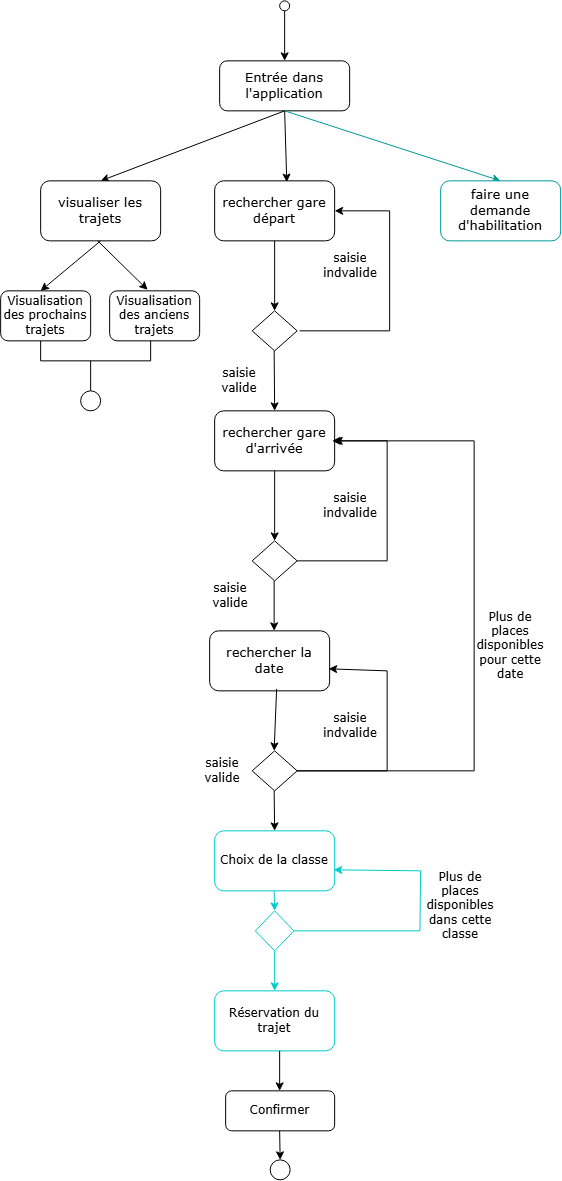
\includegraphics[width=\textwidth,height=0.62\textheight,keepaspectratio]{images/diagramme_client.png}
  \caption{Diagramme d'activité du client}\label{fig:act-client}
\end{figure}

\begin{figure}[H]
  \centering
  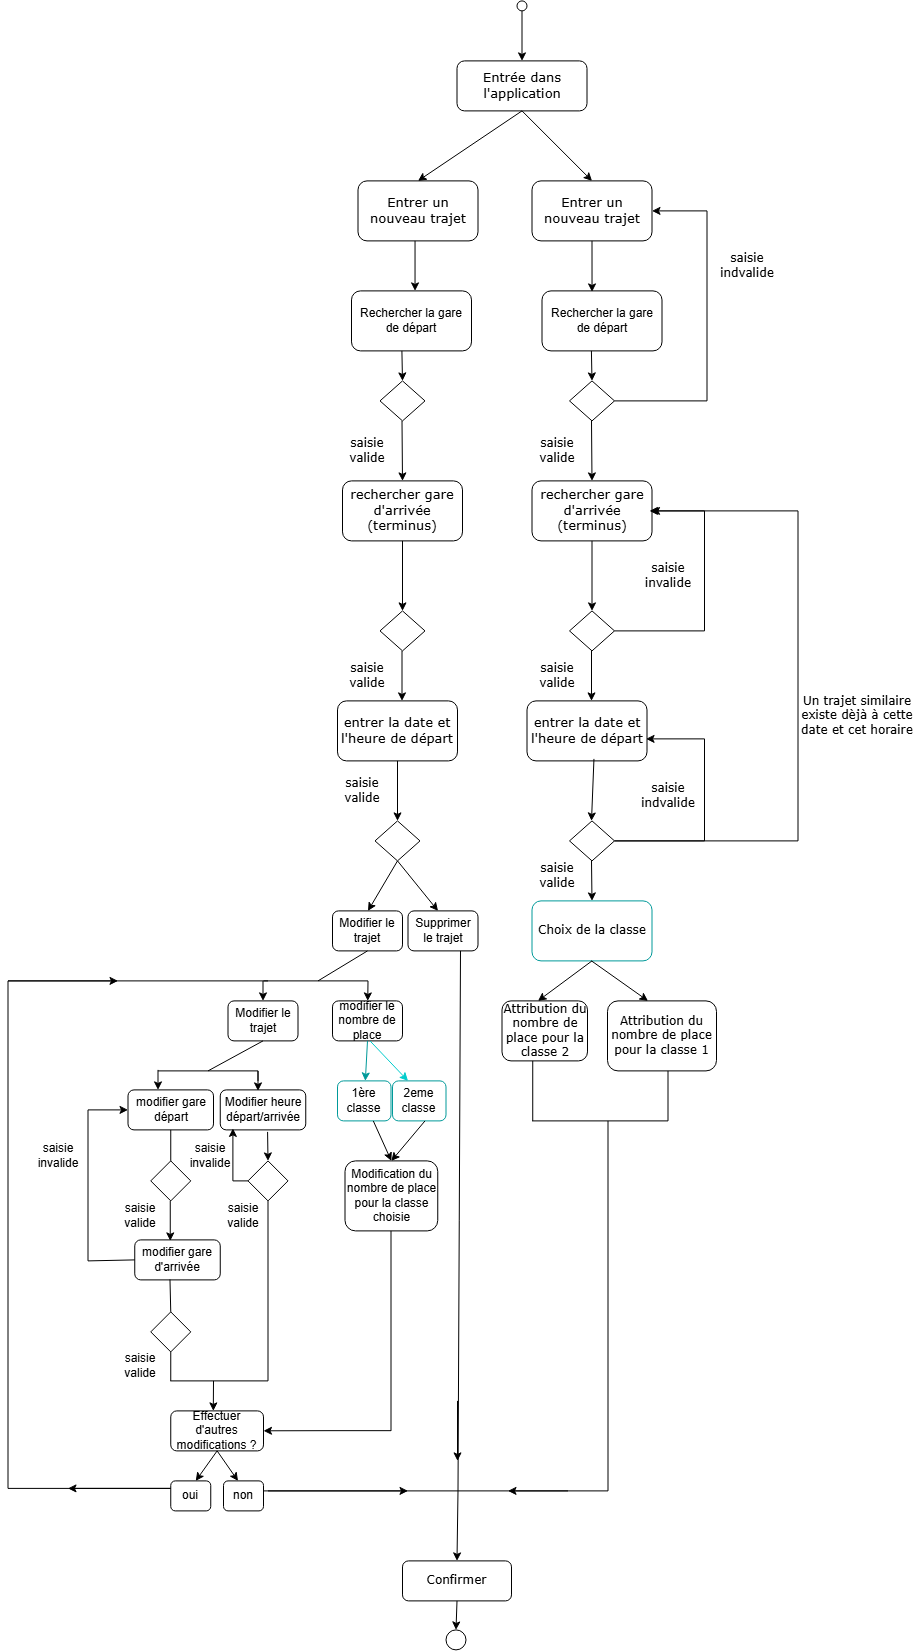
\includegraphics[width=\textwidth,height=0.62\textheight,keepaspectratio]{images/diagramme_collaborateur.png}
  \caption{Diagramme d'activité du collaborateur}\label{fig:act-collab}
\end{figure}

\begin{figure}[H]
  \centering
  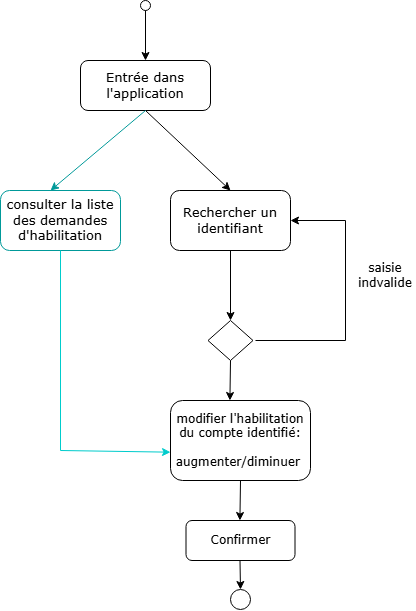
\includegraphics[width=\textwidth,height=0.38\textheight,keepaspectratio]{images/diagramme_administrateur.png}
  \caption{Diagramme d'activité de l'administrateur}\label{fig:act-admin}
\end{figure}

\subsection{Architecture de l'application}

L'application suit une architecture en couches (figure~\ref{fig:architecture}). Chaque couche
n'appelle que la couche située en dessous d'elle.

\begin{itemize}[itemsep=1pt]
  \item \textbf{Contrôleurs} (\code{controller/}) : points d'entrée HTTP (FastAPI). Ils valident les
        données reçues (schémas Pydantic), identifient l'utilisateur à partir de son jeton,
        vérifient son grade et traduisent les erreurs métier en codes HTTP.
  \item \textbf{Services} (\code{classes\_service/}) : règles métier (droits, cohérence des
        données, calcul des durées, des places et des prix). Ils lèvent des erreurs Python
        (\code{ValueError}) et ne connaissent pas HTTP.
  \item \textbf{DAO} (\code{classes\_DAO/}) : seules classes à exécuter du SQL ; elles transforment
        les lignes de la base en objets métier.
  \item \textbf{Objets métier} (\code{classes\_objets/}) : \code{Utilisateur}, \code{Client},
        \code{Gare}, \code{Ligne}, \code{Train}, \code{Trajet}, \code{Reservation}. Ils circulent
        entre les trois couches.
  \item \textbf{Utilitaires} (\code{utils/}) : connexion à la base (singleton), sécurité (hachage,
        vérification du jeton), client de l'API SNCF, journalisation.
\end{itemize}

\begin{figure}[H]
\centering
\begin{tikzpicture}[node distance=0.55cm and 1.1cm]
  % Clients
  \node[boite, minimum width=5.6cm] (front) {\textbf{Clients de l'API}\\Swagger (\code{/docs}) ou interface Streamlit};
  % Backend
  \node[couche, below=1.25cm of front] (ctrl) {\textbf{Contrôleurs}\\routes FastAPI, schémas Pydantic};
  \node[couche, below=of ctrl] (serv) {\textbf{Services}\\règles métier};
  \node[couche, below=of serv] (dao) {\textbf{DAO}\\requêtes SQL};
  \node[boite, right=1.3cm of serv, minimum width=3.2cm, text width=3.1cm, font=\scriptsize] (obj)
       {\textbf{Objets métier}\\Utilisateur, Client, Gare, Ligne, Train, Trajet, Reservation};
  \node[boite, left=1.3cm of serv, minimum width=2.9cm, text width=2.8cm, font=\scriptsize] (sncfc)
       {\textbf{SncfClient}\\\code{sncf\_client.py}};
  \begin{scope}[on background layer]
    \node[draw=ensai, dashed, rounded corners=4pt, fill=ensai!5, inner sep=8pt,
          fit=(ctrl)(serv)(dao)(obj)(sncfc)] (back) {};
  \end{scope}
  \node[font=\small\bfseries, ensaifonce, anchor=north east] at (back.north east) {Backend (Python)};
  % Externes
  \node[boite, below=1.25cm of dao, minimum width=4.6cm] (bdd) {\textbf{PostgreSQL}\\utilisateurs, gares, lignes,\\trains, trajets, réservations};
  \node[boite, minimum width=3.2cm] (sncf) at (sncfc |- bdd) {\textbf{API SNCF}\\\code{api.sncf.com}};

  % Flux
  \draw[fleche] ([xshift=-6mm]front.south) -- node[etiq, left]{requête HTTP(S)} ([xshift=-6mm]ctrl.north);
  \draw[retour] ([xshift=6mm]ctrl.north) -- node[etiq, right]{réponse JSON} ([xshift=6mm]front.south);
  \draw[fleche] (ctrl) -- (serv);
  \draw[fleche] (serv) -- (dao);
  \draw[fleche] (serv) -- (sncfc);
  \draw[fleche] ([xshift=-6mm]dao.south) -- node[etiq, left]{SQL (psycopg2)} ([xshift=-6mm]bdd.north);
  \draw[retour] ([xshift=6mm]bdd.north) -- node[etiq, right]{lignes} ([xshift=6mm]dao.south);
  \draw[fleche] ([xshift=-5mm]sncfc.south) -- node[etiq, left, align=center]{requête\\HTTP(S)} ([xshift=-5mm]sncf.north);
  \draw[retour] ([xshift=5mm]sncf.north) -- node[etiq, right, align=center]{réponse\\JSON} ([xshift=5mm]sncfc.south);
  \draw[dependance] (obj.west) -- (serv.east);
  \draw[dependance] (obj.north west) -- (ctrl.east);
  \draw[dependance] (obj.south west) -- (dao.east);
\end{tikzpicture}
\caption{Diagramme d'architecture (les flèches pointillées grises indiquent l'utilisation des objets métier)}\label{fig:architecture}
\end{figure}

\paragraph{Choix de synchronisation avec l'API SNCF.}
Interroger l'API SNCF à chaque lettre tapée rendrait l'autocomplétion lente et consommerait le
quota de requêtes. Les gares sont donc \textbf{importées à la demande} par un collaborateur
(route \route{POST /collaborateur/gares/importer}), puis conservées en base avec leur identifiant
SNCF. L'autocomplétion est alors une simple requête SQL sur notre base. Une ré-importation met à
jour une gare existante au lieu de la dupliquer (contrainte d'unicité sur l'identifiant SNCF).

\subsection{Diagramme de classes}

\paragraph{Objets métier.}
Conformément aux retours reçus, les associations entre classes sont des \textbf{références
d'objets} et non des identifiants (figure~\ref{fig:classes}). Le grade d'un utilisateur est un
attribut : les classes \code{Collaborateur} et \code{Administrateur} du dossier d'analyse ont été
supprimées, car elles n'apportaient aucun comportement propre. Seule la classe \code{Client} est
conservée, parce qu'une réservation appartient obligatoirement à un client. Les attributs
\code{places\_restantes\_*} et \code{detail\_prix\_*} d'un trajet sont calculés par le service lors
d'une recherche (F5) et ne sont pas stockés.

\begin{figure}[H]
\centering
\resizebox{\textwidth}{!}{%
\begin{tikzpicture}[node distance=1.0cm and 1.4cm]
  \node[classe] (uti) {\textbf{Utilisateur}
    \nodepart{second} id : int\\ nom\_utilisateur : str (15 car. max)\\ mdp : str (haché)\\
    grade : str (CLIENT, COLLABORATEUR, ADMIN)\\ token : str};
  \node[classe, below=1.4cm of uti] (cli) {\textbf{Client}
    \nodepart{second} grade = CLIENT};
  \node[classe, right=1.6cm of cli] (res) {\textbf{Reservation}
    \nodepart{second} id\_reservation : int\\ client : \textbf{Client}\\ trajet : \textbf{Trajet}\\
    place : str (numéro)\\ classe : int (1 ou 2)\\ prix : float};
  \node[classe, right=1.6cm of res] (traj) {\textbf{Trajet}
    \nodepart{second} id\_trajet : int\\ heure\_depart : datetime\\ heure\_arrivee : datetime\\
    ligne : \textbf{Ligne}\\ train : \textbf{Train}\\ tarif\_base : float\\ temps\_trajet : int (min)\\
    \textit{places\_restantes\_premiere, \_seconde}\\ \textit{detail\_prix\_premiere, \_seconde}};
  \node[classe, above=1.2cm of traj] (train) {\textbf{Train}
    \nodepart{second} id\_train : int\\ type\_train : str\\ places\_premieres : int\\
    places\_secondes : int\\ num\_train : int};
  \node[classe, right=1.5cm of traj] (lig) {\textbf{Ligne}
    \nodepart{second} id\_ligne : int\\ gare\_depart : \textbf{Gare}\\ gare\_arrivee : \textbf{Gare}};
  \node[classe, above=1.2cm of lig] (gare) {\textbf{Gare}
    \nodepart{second} id\_gare : int\\ nom : str\\ ville : str\\ id\_sncf : str};

  \draw[heritage] (cli) -- (uti);
  \draw[assoc] (res.west) -- node[etiq, above]{1} node[etiq, below, pos=0.85]{0..*} (cli.east);
  \draw[assoc] (res.east) -- node[etiq, above, pos=0.85]{1} node[etiq, below, pos=0.15]{0..*} (traj.west);
  \draw[assoc] (traj.north) -- node[etiq, right, pos=0.85]{0..1} node[etiq, right, pos=0.15]{0..*} (train.south);
  \draw[assoc] (traj.east) -- node[etiq, above, pos=0.85]{1} node[etiq, below, pos=0.15]{0..*} (lig.west);
  \draw[-{Diamond[open,length=3mm,width=2.4mm]}, thick] (gare.south) -- node[etiq, right, pos=0.2]{2} node[etiq, right, pos=0.8]{0..*} (lig.north);
\end{tikzpicture}}
\caption{Diagramme de classes des objets métier}\label{fig:classes}
\end{figure}

\paragraph{Services et DAO.}
Chaque objet dispose d'une classe DAO pour son accès aux données. Les services regroupent les règles
métier ; les dépendances entre services suivent celles des objets : la réservation dépend du trajet,
qui dépend de la ligne, du train et des gares. Le tableau~\ref{tab:services} liste les méthodes
principales.

\begin{table}[H]
\centering\small
\begin{tabularx}{\textwidth}{@{}l Y@{}}
\toprule
\textbf{Classe} & \textbf{Méthodes principales} \\
\midrule
\code{UtilisateurService}    & \code{creer\_compte}, \code{login}, \code{changer\_mdp}, \code{rechercher} \\
\code{AdministrateurService} & \code{recherche\_compte}, \code{gerer\_habilitation} \\
\code{CollaborateurService}  & \code{creer\_ligne}, \code{modifier\_ligne}, \code{supprimer\_ligne},
                               \code{creer\_trajet}, \code{modifier\_trajet}, \code{supprimer\_trajet},
                               \code{creer\_train}, \code{modifier\_capacite}, \code{importer\_gares} \\
\code{GareService}           & \code{rechercher} (autocomplétion), \code{importer} (API SNCF) \\
\code{LigneService}          & \code{creer}, \code{rechercher}, \code{trouver\_par\_id}, \code{modifier}, \code{supprimer} \\
\code{TrainService}          & \code{creer}, \code{trouver\_par\_id}, \code{trouver\_train\_par\_num},
                               \code{modifier\_capacite}, \code{supprimer} \\
\code{TrajetService}         & \code{creer}, \code{modifier}, \code{supprimer}, \code{rechercher},
                               \code{places\_libres}, \code{ajouter\_places\_restantes}, \code{ajouter\_detail\_prix} \\
\code{ReservationService}    & \code{creer} (vérification ou attribution de la place), \code{annuler},
                               \code{historique\_par\_client} \\
\midrule
DAO & \code{UtilisateurDAO}, \code{GareDAO}, \code{LigneDAO}, \code{TrainDAO}, \code{TrajetDAO},
      \code{ReservationDAO} : création, lecture, mise à jour, suppression, plus des requêtes
      dédiées (recherche de trajets, places réservées par trajet, capacité minimale d'un train) \\
\bottomrule
\end{tabularx}
\caption{Classes de la couche service et de la couche DAO}\label{tab:services}
\end{table}

\subsection{Base de données}\label{sec:bdd}

La base compte six tables (figure~\ref{fig:bdd}). Tous les comptes sont stockés dans une seule table
\code{utilisateurs} et distingués par la colonne \code{grade} : changer le grade d'un compte ne
demande ainsi qu'une mise à jour.

\begin{figure}[H]
\centering
\resizebox{\textwidth}{!}{%
\begin{tikzpicture}[node distance=1.0cm and 1.5cm]
  \node[tablebdd] (u) {\textbf{utilisateurs}
    \nodepart{second} \underline{id} SERIAL\\ nom\_utilisateur VARCHAR \textit{UNIQUE}\\ mdp VARCHAR\\
    grade VARCHAR\\ date\_inscription DATE\\ token\_acces VARCHAR};
  \node[tablebdd, right=1.8cm of u] (r) {\textbf{reservations}
    \nodepart{second} \underline{id\_reservation} SERIAL\\ \#id\_client INT\\ \#id\_trajet INT\\
    place VARCHAR\\ classe INT\\ prix FLOAT\\ \textit{UNIQUE (id\_trajet, classe, place)}};
  \node[tablebdd, right=1.8cm of r] (t) {\textbf{trajets}
    \nodepart{second} \underline{id\_trajet} SERIAL\\ \#id\_ligne INT\\ \#id\_train INT\\
    heure\_depart TIMESTAMP\\ heure\_arrivee TIMESTAMP\\ temps\_trajet INT\\ tarif\_base FLOAT};
  \node[tablebdd, above=1.1cm of t] (tr) {\textbf{trains}
    \nodepart{second} \underline{id\_train} SERIAL\\ type\_train VARCHAR\\ places\_premieres INT\\
    places\_secondes INT\\ num\_train INT \textit{UNIQUE}};
  \node[tablebdd, right=1.8cm of t] (l) {\textbf{lignes}
    \nodepart{second} \underline{id\_ligne} SERIAL\\ \#id\_gare\_depart INT\\ \#id\_gare\_arrivee INT\\
    \#id\_collaborateur INT};
  \node[tablebdd, above=1.1cm of l] (g) {\textbf{gares}
    \nodepart{second} \underline{id\_gare} SERIAL\\ id\_sncf VARCHAR \textit{UNIQUE}\\ nom VARCHAR\\ ville VARCHAR};

  \draw[assoc] (r.west) -- node[etiq, above]{\#id\_client} (u.east);
  \draw[assoc] (r.east) -- node[etiq, above]{\#id\_trajet} (t.west);
  \draw[assoc] (t.north) -- node[etiq, right]{\#id\_train} (tr.south);
  \draw[assoc] (t.east) -- node[etiq, above]{\#id\_ligne} (l.west);
  \draw[assoc] ([xshift=-4mm]l.north) -- node[etiq, left]{départ} ([xshift=-4mm]g.south);
  \draw[assoc] ([xshift=4mm]l.north) -- node[etiq, right]{arrivée} ([xshift=4mm]g.south);
  \draw[assoc] (l.south) .. controls +(0,-2.6) and +(0,-2.6) .. node[etiq, below]{\#id\_collaborateur} (u.south);
\end{tikzpicture}}
\caption{Modèle physique de la base de données (\underline{clé primaire}, \#clé étrangère)}\label{fig:bdd}
\end{figure}

\paragraph{Places restantes.}
Suite à la remarque sur le dossier d'analyse, les colonnes \code{places\_restantes} et \code{tarif}
de la table \code{reservations} ont été supprimées. Le nombre de places restantes est une propriété
du \textbf{trajet} : il vaut, pour chaque classe, la capacité du train du trajet moins le nombre de
réservations du trajet dans cette classe. Il est calculé à la volée par une seule requête groupée
(\code{GROUP BY id\_trajet, classe}) plutôt que stocké. Cela évite toute incohérence : une
réservation ou une annulation met automatiquement à jour l'affichage, sans valeur à maintenir.

\paragraph{Contraintes d'intégrité.}
Les règles critiques sont garanties par la base elle-même, et pas seulement par le code :
\begin{itemize}[nosep]
  \item \code{UNIQUE (id\_trajet, classe, place)} : une place n'est vendue qu'une fois, même si deux
        clients réservent au même instant ;
  \item \code{nom\_utilisateur UNIQUE} : deux comptes ne peuvent pas avoir le même nom ;
  \item \code{id\_sncf UNIQUE} : une gare n'est importée qu'une fois ;
  \item clés étrangères : un trajet ne peut pas être supprimé s'il a des réservations, ni une ligne
        si elle a des trajets.
\end{itemize}
La base est en troisième forme normale : chaque attribut est atomique et dépend uniquement de la clé
de sa table (la durée et la capacité, par exemple, sont stockées une seule fois, dans
\code{trajets} et \code{trains}).

\subsection{Diagrammes de séquence}

Les deux diagrammes suivants précisent, pour chaque message, la route ou la méthode appelée, y
compris les points d'accès de l'API SNCF.

\paragraph{Recherche d'une gare.}
La figure~\ref{fig:seq-gare} montre les deux temps du fonctionnement : l'import des gares par un
collaborateur (appel à l'API SNCF), puis l'autocomplétion par n'importe quel utilisateur connecté
(requête sur notre base uniquement).

\begin{figure}[H]
\centering
\resizebox{\textwidth}{!}{%
\begin{tikzpicture}[x=1cm,y=1.3cm, font=\scriptsize]
  % Participants
  \foreach \x/\nom/\txt in {0/U/Utilisateur, 3.8/C/{utilisateur\_controller\\collaborateur\_controller},
                        7.6/S/GareService, 10.6/K/SncfClient, 13.6/A/API SNCF,
                        16.6/D/GareDAO, 19.6/B/PostgreSQL}{
    \node[boite, font=\scriptsize, minimum height=0.8cm] (\nom) at (\x,0) {\txt};
    \draw[dashed, gris] (\nom.south) -- (\x,-12.3);
  }
  % --- Phase 1 : import ---
  \node[font=\scriptsize\bfseries, ensaifonce, anchor=west] at (-0.8,-0.75) {1. Import (collaborateur)};
  \draw[fleche] (0,-1.65) -- node[etiq, above]{POST /collaborateur/gares/importer?q=Rennes} (3.8,-1.65);
  \draw[fleche] (3.8,-2.1) -- node[etiq, above]{importer("Rennes")} (7.6,-2.1);
  \draw[fleche] (7.6,-2.7) -- node[etiq, above]{rechercher\_gares("Rennes")} (10.6,-2.7);
  \draw[fleche] (10.6,-3.3) -- node[etiq, above, align=center]{GET /coverage/sncf/places\\?type[]=stop\_area\&q=Rennes} (13.6,-3.3);
  \draw[retour] (13.6,-4.1) -- node[etiq, above]{JSON : places (id, name, communes)} (10.6,-4.1);
  \draw[retour] (10.6,-4.7) -- node[etiq, above]{liste [id\_sncf, nom, ville]} (7.6,-4.7);
  \draw[fleche] (7.6,-5.3) -- node[etiq, above]{creer\_ou\_mettre\_a\_jour(gare)} (16.6,-5.3);
  \draw[fleche] (16.6,-5.9) -- node[etiq, above, align=center]{INSERT INTO gares \dots\\ON CONFLICT (id\_sncf) DO UPDATE} (19.6,-5.9);
  \draw[retour] (7.6,-6.6) -- node[etiq, above]{gares importées} (3.8,-6.6);
  \draw[retour] (3.8,-7.1) -- node[etiq, above]{200 : liste JSON des gares} (0,-7.1);
  % --- Phase 2 : autocompletion ---
  \node[font=\scriptsize\bfseries, ensaifonce, anchor=west] at (-0.8,-7.65) {2. Autocomplétion (tout utilisateur connecté)};
  \draw[fleche] (0,-8.55) -- node[etiq, above]{GET /utilisateur/gares?nom=Ren} (3.8,-8.55);
  \draw[fleche] (3.8,-9.0) -- node[etiq, above]{rechercher("Ren", None)} (7.6,-9.0);
  \draw[fleche] (7.6,-9.6) -- node[etiq, above]{rechercher(nom, ville)} (16.6,-9.6);
  \draw[fleche] (16.6,-10.2) -- node[etiq, above]{SELECT \dots{} WHERE nom ILIKE 'Ren\%'} (19.6,-10.2);
  \draw[retour] (16.6,-10.9) -- node[etiq, above]{liste de Gare} (7.6,-10.9);
  \draw[retour] (7.6,-11.4) -- (3.8,-11.4);
  \draw[retour] (3.8,-11.9) -- node[etiq, above]{200 : Rennes, Rennes Beaulieu Chimie\dots} (0,-11.9);
\end{tikzpicture}}
\caption{Diagramme de séquence : import et recherche d'une gare}\label{fig:seq-gare}
\end{figure}

\paragraph{Création d'un trajet.}
La figure~\ref{fig:seq-trajet} montre la création d'un trajet par un collaborateur. Les
vérifications locales (ligne, train, doublon) sont faites \textbf{avant} l'appel à l'API SNCF, pour
ne pas consommer de requête inutilement.

\begin{figure}[H]
\centering
\resizebox{\textwidth}{!}{%
\begin{tikzpicture}[x=1cm,y=1.3cm, font=\scriptsize]
  \foreach \x/\nom/\txt in {0/U/Collaborateur, 3.9/C/collaborateur\_controller, 7.6/S/TrajetService,
                        11.2/K/SncfClient, 14.2/A/API SNCF, 17.4/D/{LigneDAO, TrainDAO\\TrajetDAO}, 20.4/B/PostgreSQL}{
    \node[boite, font=\scriptsize, minimum height=0.8cm] (\nom) at (\x,0) {\txt};
    \draw[dashed, gris] (\nom.south) -- (\x,-10.4);
  }
  \draw[fleche] (0,-1.2) -- node[etiq, above, align=center]{POST /collaborateur/trajets\\\{id\_ligne, id\_train, heure\_depart, tarif\_base\}} (3.9,-1.2);
  \node[etiq, anchor=west, align=left, text width=2.6cm] at (4.0,-1.95) {vérifie le jeton\\et le grade};
  \draw[fleche] (3.9,-2.6) -- node[etiq, above]{creer(id\_ligne, id\_train, \dots)} (7.6,-2.6);
  \draw[fleche] (7.6,-3.2) -- node[etiq, above, align=center]{trouver\_par\_id (ligne, train)\\rechercher (doublon à la même heure)} (17.4,-3.2);
  \draw[fleche] (17.4,-3.8) -- node[etiq, above]{SELECT \dots} (20.4,-3.8);
  \draw[retour] (17.4,-4.4) -- node[etiq, above]{Ligne (avec ses Gare), Train, aucun doublon} (7.6,-4.4);
  \draw[fleche] (7.6,-5.0) -- node[etiq, above]{duree\_trajet(id\_sncf départ, id\_sncf arrivée, date)} (11.2,-5.0);
  \draw[fleche] (11.2,-5.6) -- node[etiq, above, align=center]{GET /coverage/sncf/journeys\\?from=\dots\&to=\dots\&datetime=\dots} (14.2,-5.6);
  \draw[retour] (14.2,-6.4) -- node[etiq, above]{JSON : journeys[].duration} (11.2,-6.4);
  \draw[retour] (11.2,-7.0) -- node[etiq, above]{durée minimale (s)} (7.6,-7.0);
  \draw[fleche] (7.6,-7.6) -- node[etiq, above]{creer(trajet) : arrivée = départ + durée} (17.4,-7.6);
  \draw[fleche] (17.4,-8.2) -- node[etiq, above]{INSERT INTO trajets \dots{} RETURNING id\_trajet} (20.4,-8.2);
  \draw[retour] (17.4,-8.8) -- node[etiq, above]{Trajet (id\_trajet)} (7.6,-8.8);
  \draw[retour] (7.6,-9.4) -- (3.9,-9.4);
  \draw[retour] (3.9,-10.0) -- node[etiq, above, align=center]{201 : id\_trajet, heure\_arrivee,\\temps\_trajet (ex. 77 min)} (0,-10.0);
\end{tikzpicture}}
\caption{Diagramme de séquence : création d'un trajet}\label{fig:seq-trajet}
\end{figure}

% ============================ 4. IMPLEMENTATION =======================
\clearpage
\section{Implémentation}\label{sec:implementation}

\subsection{Points d'accès exposés par notre API}

L'API expose 22 routes, regroupées par profil dans le Swagger (tableau~\ref{tab:routes}). Toutes les
routes, sauf la connexion et la création de compte, exigent l'en-tête \code{X-Auth-Token}.

\begingroup\footnotesize
\begin{longtable}{@{}l p{7.0cm} l >{\raggedright\arraybackslash}p{3.3cm}@{}}
\caption{Routes exposées par l'API}\label{tab:routes}\\
\toprule
\textbf{Méthode} & \textbf{Route} & \textbf{Accès} & \textbf{Rôle} \\
\midrule
\endfirsthead
\toprule
\textbf{Méthode} & \textbf{Route} & \textbf{Accès} & \textbf{Rôle} \\
\midrule
\endhead
\bottomrule
\endfoot
POST   & \route{/login/}                                    & public        & Connexion, renvoie le jeton \\
POST   & \route{/utilisateur/comptes}                       & public        & Créer un compte client \\
PUT    & \route{/utilisateur/mot-de-passe}                  & connecté      & Changer son mot de passe \\
GET    & \route{/utilisateur/gares?nom=\&ville=}            & connecté      & Autocomplétion des gares \\
GET    & \route{/utilisateur/trajets}\newline\route{?gare\_depart=\&gare\_arrivee=\&date\_voyage=} & connecté & Rechercher des trajets (F4, F5) \\
GET    & \route{/utilisateur/trajets/\{id\_trajet\}/places} & connecté      & Places libres par classe \\
GET    & \route{/utilisateur/trains/\{num\_train\}}         & connecté      & Consulter un train \\
POST   & \route{/utilisateur/reservations}                  & CLIENT        & Réserver (FO1, FO2) \\
GET    & \route{/utilisateur/reservations}                  & CLIENT        & Ses réservations \\
DELETE & \route{/utilisateur/reservations/\{id\_reservation\}} & CLIENT     & Annuler une réservation \\
POST   & \route{/collaborateur/gares/importer?q=}           & COLLABORATEUR & Importer des gares SNCF \\
POST   & \route{/collaborateur/trains}                      & COLLABORATEUR & Créer un train \\
PUT    & \route{/collaborateur/trains/\{num\_train\}}       & COLLABORATEUR & Modifier sa capacité \\
POST   & \route{/collaborateur/lignes}                      & COLLABORATEUR & Créer une ligne (F2) \\
PUT    & \route{/collaborateur/lignes/\{id\_ligne\}}        & COLLABORATEUR & Modifier une ligne \\
DELETE & \route{/collaborateur/lignes/\{id\_ligne\}}        & COLLABORATEUR & Supprimer une ligne \\
POST   & \route{/collaborateur/trajets}                     & COLLABORATEUR & Planifier un trajet (F3) \\
PUT    & \route{/collaborateur/trajets/\{id\_trajet\}}      & COLLABORATEUR & Modifier un trajet \\
DELETE & \route{/collaborateur/trajets/\{id\_trajet\}}      & COLLABORATEUR & Supprimer un trajet \\
GET    & \route{/admin/utilisateurs}\newline\route{?id\_utilisateur=\&nom\_utilisateur=} & ADMIN & Rechercher un compte \\
PUT    & \route{/admin/utilisateurs/\{id\}/grade}\newline\route{?nouveau\_grade=} & ADMIN   & Modifier l'habilitation \\
GET    & \route{/reset\_database}                           & ADMIN         & Réinitialiser la base \\
\end{longtable}
\endgroup

\subsection{Points d'accès consommés dans l'API SNCF}

Les appels à l'API SNCF sont regroupés dans une seule classe, \code{SncfClient}
(tableau~\ref{tab:sncf}). L'authentification se fait par le jeton fourni par la SNCF, lu dans le
fichier \code{.env} (non versionné). Chaque appel a un délai maximal de 10~secondes.

\begin{table}[H]
\centering\small
\begin{tabularx}{\textwidth}{@{}p{4.3cm} Y Y@{}}
\toprule
\textbf{Point d'accès} & \textbf{Données récupérées} & \textbf{Utilisation} \\
\midrule
\route{GET /coverage/sncf/places} \newline \code{?type[]=stop\_area} \newline \code{\&q=<texte>}
  & Pour chaque gare : identifiant SNCF (\code{stop\_area:SNCF:\dots}), nom, et commune
    (région administrative de niveau 8).
  & Import des gares dans notre base (F2), avant l'autocomplétion. \\
\route{GET /coverage/sncf/journeys} \newline \code{?from=<id>\&to=<id>} \newline \code{\&datetime=<date>}
  & Liste d'itinéraires et leur durée en secondes (\code{journeys[].duration}).
  & Durée du trajet (F3) : la plus courte est retenue. Une réponse vide ou une erreur 404 signifie
    qu'aucun itinéraire n'existe : la création est refusée. \\
\bottomrule
\end{tabularx}
\caption{Points d'accès de l'API SNCF utilisés}\label{tab:sncf}
\end{table}

\subsection{Authentification et sécurité}

\begin{itemize}[itemsep=2pt]
  \item \textbf{Mots de passe.} Ils sont hachés en SHA-256, salés avec le nom d'utilisateur. Le mot
        de passe en clair n'est jamais stocké ni renvoyé par l'API.
  \item \textbf{Jeton.} À la connexion, un jeton aléatoire (\code{secrets.token\_urlsafe}) est
        généré et enregistré. Chaque requête protégée le transmet dans l'en-tête
        \code{X-Auth-Token}, et la dépendance FastAPI \code{verif\_token} retrouve l'utilisateur
        correspondant.
  \item \textbf{Identité tirée du jeton.} Les identifiants de client et de collaborateur ont été
        retirés des requêtes : un utilisateur ne peut donc ni réserver, ni consulter, ni annuler au
        nom d'un autre, ni attribuer une ligne à un autre collaborateur. Une annulation vérifie en
        plus que la réservation appartient au client connecté.
  \item \textbf{Droits.} L'administrateur ne peut pas modifier le grade d'un autre administrateur,
        et la réinitialisation de la base vérifie le grade \emph{avant} toute action.
\end{itemize}

Les erreurs suivent une convention unique (tableau~\ref{tab:codes}) : les services lèvent des
erreurs Python, et seuls les contrôleurs les traduisent en codes HTTP.

\begin{table}[H]
\centering\small
\begin{tabularx}{\textwidth}{@{}c Y@{}}
\toprule
\textbf{Code} & \textbf{Signification} \\
\midrule
400 & Donnée invalide ou règle métier non respectée (place inexistante, classe complète, doublon\dots) \\
401 & Non connecté : jeton absent ou invalide, ou identifiants incorrects \\
403 & Connecté, mais grade insuffisant pour cette route \\
404 & Objet introuvable (trajet, ligne, train, réservation\dots) \\
422 & Requête mal formée (contrôle automatique des schémas Pydantic) \\
502 & API SNCF indisponible ou mal configurée \\
\bottomrule
\end{tabularx}
\caption{Codes d'erreur renvoyés par l'API}\label{tab:codes}
\end{table}

\subsection{Lignes et trajets}

Une ligne ne peut relier que deux gares différentes, et une même ligne ne peut pas être créée deux
fois. Les gares sont désignées par leur nom : le nom exact est prioritaire (\og Rennes \fg{}
désigne Rennes et non Rennes Beaulieu Chimie) ; un début de nom est accepté s'il ne correspond qu'à
une gare, sinon l'API répond en listant les gares possibles.

À la création ou à la modification d'un trajet, le service vérifie que la ligne et le train
existent et qu'aucun autre trajet ne part sur la même ligne à la même heure, puis calcule l'heure
d'arrivée à partir de la durée renvoyée par l'API SNCF. Un trajet ou une ligne encore utilisés
(réservations, trajets) ne peuvent pas être supprimés.

\subsection{Réservations et gestion des places}

\paragraph{Absence de surréservation.}
Une place est un numéro compris entre 1 et la capacité de la classe dans le train du trajet. Avec
la contrainte d'unicité de la base, il est impossible de vendre plus de places qu'il n'en existe,
y compris si deux clients réservent au même instant.

\paragraph{Attribution automatique.}
Si le client n'indique pas de place, le service lui attribue la plus petite place libre de la
classe choisie. Si cette place est prise par un autre client entre le calcul et l'insertion, la
base refuse l'insertion et le service recommence avec la place libre suivante (trois essais au
plus). Une place choisie explicitement n'est jamais remplacée sans l'accord du client : elle est
refusée si elle est prise.

\begin{lstlisting}
# ReservationService.creer (extrait simplifie)
attribution_auto = not place
for tentative in range(1, tentatives + 1):
    place = (self._attribuer_place(trajet, classe) if attribution_auto
             else self._verifier_place(trajet, place, classe))
    try:
        return ReservationDAO().creer(Reservation(client, trajet, place, classe, prix))
    except UniqueViolation:          # place prise entre-temps par un autre client
        if attribution_auto and tentative < tentatives:
            continue                 # on essaie la place libre suivante
        raise ValueError("Place deja reservee")
\end{lstlisting}

\paragraph{Modification de la capacité d'un train.}
Un collaborateur ne peut pas réduire la capacité d'une classe en dessous de ce qui est déjà réservé
sur les trajets à venir de ce train : ni sous le nombre de réservations, ni sous le plus grand
numéro de place réservé. Les trajets passés ne bloquent pas la modification.

\subsection{Positionnement commercial (F5)}

Le sujet laisse cette fonctionnalité libre. Nous en avons retenu deux, directement visibles dans
les résultats de recherche :
\begin{itemize}[nosep]
  \item \textbf{Places restantes}, par classe, pour chaque trajet trouvé ;
  \item \textbf{Tarification transparente} : le détail de ce que paie le client, sur le modèle
        présenté au tableau~\ref{tab:prix}.
\end{itemize}

\begin{table}[H]
\centering\small
\begin{tabular}{@{}l r r@{}}
\toprule
\textbf{Poste} & \textbf{2de classe} & \textbf{1re classe} \\
\midrule
Coût d'exploitation (50\,\% du HT)      &  9,09~\texteuro{} & 13,64~\texteuro{} \\
Péage réseau versé à SNCF Réseau (35\,\% du HT) &  6,36~\texteuro{} &  9,54~\texteuro{} \\
Marge de la compagnie (reste du HT)     &  2,73~\texteuro{} &  4,09~\texteuro{} \\
TVA (10\,\%)                            &  1,82~\texteuro{} &  2,73~\texteuro{} \\
\midrule
\textbf{Prix payé}                      & \textbf{20,00~\texteuro{}} & \textbf{30,00~\texteuro{}} \\
\bottomrule
\end{tabular}
\caption{Détail du prix renvoyé pour un trajet au tarif de base de 20~\texteuro{}}\label{tab:prix}
\end{table}

Les calculs sont faits en centimes, la marge absorbant les arrondis : la somme des postes est
toujours exactement égale au prix payé (propriété vérifiée par les tests sur 18 montants). Les
pourcentages sont des hypothèses de la compagnie, regroupées dans un seul module
(\code{tarification.py}) pour pouvoir être modifiées facilement.

\subsection{Interface web (bonus)}

Le sujet n'exige pas d'interface : le Swagger suffit. Une interface Streamlit a toutefois été
développée pour la démonstration. Elle appelle uniquement l'API, comme le feraient les webmasters
de l'entreprise, et affiche les pages selon le grade de l'utilisateur connecté : recherche avec un
panneau des départs (horaires, durée, prix, places restantes, détail du prix), réservation avec
liste des places libres, gestion des gares, lignes, trains et trajets, et administration des
comptes.

% ============================ 5. QUALITE ===============================
\section{Assurance qualité}\label{sec:qualite}

\subsection{Tests automatisés}

Les tests sont écrits avec \code{pytest}. La base de données et l'API SNCF y sont
\textbf{simulées} grâce à \code{unittest.mock} : les tests ne dépendent ni d'une connexion ni de
données existantes, et
s'exécutent en quelques secondes. Les routes sont testées par de vraies requêtes HTTP grâce au
\code{TestClient} de FastAPI. Chaque test suit la structure \emph{GIVEN}, \emph{WHEN},
\emph{THEN} et couvre le cas nominal et les cas d'erreur.

\begin{table}[H]
\centering\small
\begin{tabular}{@{}l l r@{}}
\toprule
\textbf{Dossier} & \textbf{Ce qui est testé} & \textbf{Tests} \\
\midrule
\code{tests/test\_objets}              & classes métier, client de l'API SNCF          &  39 \\
\code{tests/tests\_DAO}                & requêtes SQL et transformation en objets      &  95 \\
\code{tests/tests\_service}            & règles métier, tarification                   & 186 \\
\code{tests/test\_controller\_optionel}& routes HTTP : codes de retour, sécurité       &  70 \\
\midrule
\textbf{Total}                         &                                                & \textbf{390} \\
\bottomrule
\end{tabular}
\caption{Répartition des tests automatisés (tous réussis)}
\end{table}

La couverture du code, mesurée avec \code{pytest-cov}, atteint \textbf{85\,\%} : 93\,\% pour les
objets métier, 90\,\% pour les services, 86\,\% pour les contrôleurs, 82\,\% pour les DAO et
100\,\% pour les schémas. Les utilitaires (68\,\%) contiennent la configuration des journaux et la
réinitialisation de la base, qui ne sont pas testées unitairement.

\subsection{Tests de bout en bout}

Les tests automatisés simulent la base ; nous avons donc aussi vérifié l'application réelle. Un
script rejoue le parcours complet par de vraies requêtes HTTP, sur une base PostgreSQL et avec la
vraie API SNCF. Il s'exécute dans un \textbf{schéma de test séparé}, pour ne jamais modifier les
données de travail.

\begin{itemize}[nosep]
  \item \textbf{API :} 56 vérifications (comptes et droits, import des gares, lignes, trains,
        trajets avec durée réelle de 77 minutes entre Rennes et Nantes, réservations, places
        restantes, contrôles de capacité, suppressions) : \textbf{56 réussies}.
  \item \textbf{Interface :} 27 vérifications avec l'outil de test officiel de Streamlit
        (\code{AppTest}) : affichage du détail des prix, liste des places libres, réservation
        automatique puis choisie, classe complète : \textbf{27 réussies}.
\end{itemize}

\paragraph{Défauts détectés et corrigés.}
Cette démarche a révélé plusieurs défauts, corrigés avant le rendu et désormais couverts par un test :
\begin{itemize}[nosep]
  \item la réservation et l'historique renvoyaient une erreur 500 ;
  \item un client pouvait annuler la réservation d'un autre client ;
  \item n'importe quel compte connecté pouvait réinitialiser la base ;
  \item une ligne pouvait être attribuée à un autre collaborateur ;
  \item aucune limite de places n'empêchait la surréservation ;
  \item l'absence du jeton SNCF provoquait une erreur 500 au lieu d'une 502.
\end{itemize}

\subsection{Pratiques de développement}

\begin{itemize}[itemsep=1pt]
  \item \textbf{Documentation.} Chaque méthode a une \emph{docstring} (paramètres, retour,
        exceptions). Le Swagger est généré automatiquement et décrit chaque route. Le README
        explique l'installation, le lancement, les comptes de test et les règles métier.
  \item \textbf{Journalisation.} Chaque requête HTTP et chaque appel de méthode décorée par
        \code{@log} sont tracés dans un fichier de logs, avec les erreurs de base de données.
  \item \textbf{Configuration.} Les mots de passe de la base et le jeton SNCF sont dans un fichier
        \code{.env}, exclu de Git.
  \item \textbf{Reproductibilité.} Les versions des dépendances sont figées (\code{uv.lock}) ; la
        base se recrée à l'identique à partir de \code{init\_bdd.sql} et \code{admin.sql}.
  \item \textbf{Git.} Une branche par évolution, des messages de commit décrivant le changement, et
        une fusion dans \code{main} uniquement lorsque tous les tests passent.
\end{itemize}

% ============================ 6. GUIDE ================================
\section{Guide d'utilisation : un cas concret}\label{sec:guide}

\paragraph{Lancement.} Depuis la racine du dépôt (le fichier \code{backend/.env} doit être rempli) :
\begin{lstlisting}[language=bash]
uv sync --project backend
cd backend && uv run python -m src.utils.reset_bdd && cd ..   # premiere fois
uv run --project backend python backend/main.py                 # API : http://127.0.0.1:5000/docs
uv run --project frontend streamlit run frontend/app.py         # interface (optionnelle)
\end{lstlisting}

Les comptes de test sont \code{admin} / \code{123}, \code{collaborateur} / \code{456} et
\code{client} / \code{789}. Le tableau~\ref{tab:scenario} déroule un scénario complet, avec les
réponses obtenues lors de nos tests sur PostgreSQL.

\begin{table}[H]
\centering\small
\begin{tabularx}{\textwidth}{@{}c l Y@{}}
\toprule
\textbf{Étape} & \textbf{Action} & \textbf{Résultat} \\
\midrule
1 & Le collaborateur importe \og Rennes \fg{} et \og Nantes \fg & Les gares de ces villes sont enregistrées
    avec leur identifiant SNCF. \\
2 & Il crée un train TER n\textsuperscript{o}~857 (2 places en 1re, 3 en 2de) & 201 : train créé. \\
3 & Il crée la ligne Rennes $\rightarrow$ Nantes & 201 : ligne n\textsuperscript{o}~1. \\
4 & Il planifie un trajet le 20/11/2026 à 8h30, à 20~\texteuro{} & 201 : durée de 77 min calculée par l'API SNCF,
    arrivée à 9h47. \\
5 & Le client cherche Rennes $\rightarrow$ Nantes le 20/11 & Le trajet s'affiche avec 2 places en 1re,
    3 en 2de, et le détail du prix. \\
6 & Il réserve trois fois en 2de sans choisir de place & Places 1, 2 et 3 attribuées, à 20~\texteuro{} chacune. \\
7 & Il tente une quatrième réservation en 2de & 400 : \og Ce trajet est complet en seconde classe \fg. \\
8 & Il réserve en 1re classe & Place 1 attribuée, à 30~\texteuro{}. \\
9 & Un autre client tente d'annuler une de ces réservations & 400 : \og Cette réservation appartient à
    un autre client \fg. \\
10 & Le collaborateur réduit la 2de classe du train à 1 place & 400 : les réservations à venir en
    demandent au moins 3. \\
\bottomrule
\end{tabularx}
\caption{Scénario d'utilisation et réponses de l'API}\label{tab:scenario}
\end{table}

% ============================ 7. LIMITES ==============================
\section{Limites et perspectives}\label{sec:limites}

\paragraph{Limites connues.}
\begin{itemize}[nosep]
  \item Le jeton de connexion n'expire pas, et une nouvelle connexion remplace le jeton précédent
        (une seule session active par compte).
  \item Un collaborateur peut modifier l'horaire d'un trajet déjà réservé ; les passagers ne sont
        pas prévenus, faute de canal de communication entre clients et collaborateurs.
  \item L'API SNCF ne connaît les horaires que sur quelques semaines : au-delà, la durée retenue est
        celle des horaires actuels.
  \item Les gares ne sont mises à jour que lors d'un nouvel import par un collaborateur.
  \item Un administrateur n'a pas accès aux actions des collaborateurs ; nommer un compte
        administrateur est possible mais irréversible, puisqu'un administrateur ne peut pas être
        rétrogradé.
\end{itemize}

\paragraph{Perspectives.}
\begin{itemize}[nosep]
  \item Expiration des jetons, ou passage à un standard comme JWT ;
  \item notification des passagers lors d'une modification ou d'une suppression de trajet ;
  \item trajets avec correspondance, combinant plusieurs lignes ;
  \item tarification dynamique, fondée sur le taux de remplissage, en réutilisant le calcul des
        places restantes ;
  \item synchronisation planifiée des gares avec l'API SNCF.
\end{itemize}

% ============================ 8. CONCLUSION ===========================
\section{Conclusion}

L'API livrée couvre l'ensemble du sujet : les cinq fonctionnalités obligatoires, dont un
positionnement commercial fondé sur les places restantes et la tarification transparente, et les
deux fonctionnalités optionnelles. Elle repose sur une architecture en couches qui sépare les routes,
les règles métier et l'accès aux données, et sur une base dont les contraintes garantissent les
règles critiques, comme l'impossibilité de vendre deux fois la même place.

La qualité a été traitée comme une exigence du projet : 390 tests automatisés couvrent 85\,\% du
code, et un parcours complet a été validé sur une vraie base avec la vraie API SNCF. Ces tests ont
mis en évidence des failles de sécurité et des erreurs de logique, corrigées avant le rendu.

Le projet a enfin permis à chacun de pratiquer la modélisation UML, la conception d'une base de
données, le développement d'une API web et le travail collaboratif avec Git. Les principales
difficultés ont été la cohérence entre les couches, développées en parallèle, et l'intégration
tardive de l'API SNCF ; les comptes rendus hebdomadaires et les tests ont permis de les surmonter.

% ============================ ANNEXES =================================
\newpage
\appendix
\section{Bilans individuels}

\acompleter{Chaque membre rédige ici un bilan d'une dizaine de lignes : tâches réalisées,
difficultés rencontrées, compétences acquises, et ce qu'il ferait différemment.}

\subsection*{Adam BENAMER}
\acompleter{À compléter.}

\subsection*{Lou-Ann CLEMENT}
\acompleter{À compléter.}

\subsection*{Satya KREMER}
\acompleter{À compléter.}

\subsection*{Laurine LEROY}
\acompleter{À compléter.}

\subsection*{Nour NSIRI}
\acompleter{Proposition à relire et à personnaliser.}
En tant que référente technique, j'ai participé à la modélisation (diagrammes de cas d'utilisation
et de base de données), puis développé les DAO des réservations et des trajets. J'ai intégré l'API
SNCF : client regroupant les appels, import des gares sans doublon et autocomplétion locale, calcul
de la durée des trajets. En fin de projet, j'ai testé toutes les fonctionnalités, corrigé les failles
de sécurité (identité tirée du jeton, annulation par un autre client, réinitialisation de la base),
et implémenté la gestion des places (absence de surréservation, attribution automatique, contrôle
de la capacité) ainsi que la tarification transparente. La principale difficulté a été de garder la
cohérence entre les couches développées en parallèle ; j'en retiens l'importance des tests et
d'une convention claire de gestion des erreurs.

\subsection*{Nathan TIATIA}
\acompleter{À compléter.}

\subsection*{Bilan de groupe}
\acompleter{À compléter ensemble : fonctionnement de l'équipe, communication, ce qui a bien marché
et ce qui serait à améliorer.}

\section{Structure du dépôt}

\begin{lstlisting}[language={}]
backend/
  main.py                    application FastAPI
  data/init_bdd.sql          creation des tables
  data/admin.sql             comptes de test
  src/Classes/controller/    routes (administrateur, collaborateur, utilisateur, login)
  src/Classes/classes_service/   services (dont tarification.py)
  src/Classes/classes_DAO/       acces aux donnees
  src/Classes/classes_objets/    objets metier
  src/schema/                modeles Pydantic
  src/utils/                 connexion BDD, securite, client SNCF, logs
  tests/                     390 tests (objets, DAO, services, routes)
frontend/                    interface Streamlit (bonus)
Dossier_analyse/             dossier d'analyse et diagrammes
suivi-folder/                comptes rendus hebdomadaires
\end{lstlisting}

\end{document}
